\chapter{Thử nghiệm hệ thống, kết luận và hướng phát triển}
\section{Thử nghiệm hệ thống}
%\newcommand{\blank}[1]{\hspace*{#1}\linebreak[0]}
Để chứng minh tính đúng đắn của hệ thống, tôi thực hiện thử nghiệm hệ thống với một câu truy vấn: Liệt kê các thiết bị trong trung tâm HPCC. \\

Câu truy vấn tương ứng trong hệ thống của tôi là:
%\begin{figure}
%	\center
%	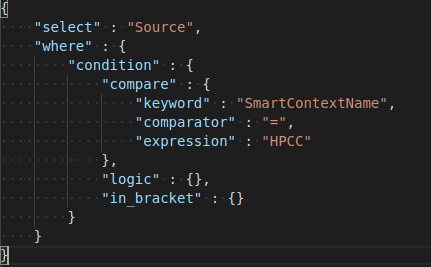
\includegraphics[scale=0.5]{image/demo_query}
%	\caption{Câu truy vấn thực nghiệm}
%\end{figure}


\{\\
\blank{1cm}"select" : "Source",\\
\blank{1cm}"where" : \{\\
\blank{2cm}"condition" : \{\\
\blank{3cm}"compare" : \{\\
\blank{4cm}    "keyword" : "SmartContextName",\\
\blank{4cm}    "comparator" : "=",\\
\blank{4cm}    "expression" : "HPCC"\\
\blank{3cm}\},\\
\blank{3cm}"logic" : \{\},\\
\blank{3cm}"in\_bracket" : \{\}\\
\blank{2cm}\}\\
\blank{1cm}\}\\
\}\\

Kết quả thu được là :\\

[\\
\blank{1cm}\{\\
\blank{2cm}'LocalId':'temperature-humidity-light\_id',\\
\blank{2cm}'SourceStatus':'active',\\
\blank{2cm}'Description':'',\\
\blank{2cm}'EndPoint':'http://192.168.0.197:8080/source',\\
\blank{2cm}'SourceId':'temperature-humidity-light\_openhab',\\
\blank{2cm}'HasMetric':[\\
\blank{3cm}'Humidity',\\
\blank{3cm}'Temperature',\\
\blank{3cm}'Light'\\
\blank{2cm}],\\
\blank{2cm}'SourceType':'thing',\\
\blank{2cm}'Label':'sensor'\\
\blank{1cm}\},\\
\blank{1cm}\{\\
\blank{2cm}'LocalId':'motion\_id',\\
\blank{2cm}'SourceStatus':'active',\\
\blank{2cm}'Description':'',\\
\blank{2cm}'EndPoint':'http://192.168.0.197:8080/source',\\
\blank{2cm}'SourceId':'motion\_openhab',\\
\blank{2cm}'HasMetric':[\\
\blank{3cm}'LedDo',\\
\blank{3cm}'LedXanh',\\
\blank{3cm}'LedVang',\\
\blank{3cm}'Motion'\\
\blank{2cm}],\\
\blank{2cm}'SourceType':'thing',\\
\blank{2cm}'Label':'sensor'\\
\blank{1cm}\},\\
\blank{1cm}\{\\
\blank{2cm}'LocalId':'temperature-humidity-light\_id',\\
\blank{2cm}'SourceStatus':'active',\\
\blank{2cm}'Description':'',\\
\blank{2cm}'EndPoint':'http://192.168.0.198:8080/source',\\
\blank{2cm}'SourceId':'temperature-humidity-light\_thingsboard',\\
\blank{2cm}'HasMetric':[\\
\blank{2cm}'b37a79a0-755c-11e9-abce-5bf295b292b2-light',\\
\blank{2cm}'b37a79a0-755c-11e9-abce-5bf295b292b2-temperature',\\
\blank{2cm}'b37a79a0-755c-11e9-abce-5bf295b292b2-humidity'\\
\blank{2cm}],\\
\blank{2cm}'SourceType':'thing',\\
\blank{2cm}'Label':'sensor'\\
\blank{1cm}\},\\
\blank{2cm}...\\
]
\clearpage

Để chứng minh hệ thống có tính khả mở, tôi thêm một nền tảng IoT là ThingsBoard vào hệ thống bằng việc viết thêm một driver để ánh xạ dữ liệu từ định dạng của ThingsBoard về định dạng của ontology. Tôi sẽ thực hiện câu truy vấn: Lấy tất cả các platform có trong trung tâm HPCC để chứng minh đã thêm được ThingsBoard vào hệ thống. \\

Câu truy vấn tương ứng trong hệ thống là:
%\begin{figure}
%	\center
%	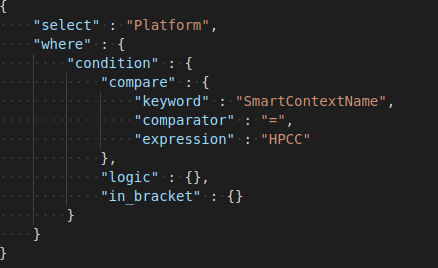
\includegraphics[scale=0.5]{image/add_thingsboard}
%	\caption{Thêm ThingsBoard vào hệ thống}
%\end{figure}

\{\\
\blank{1cm}"select" : "Platform",\\
\blank{1cm}"where" : \{\\
\blank{2cm}"condition" : \{\\
\blank{3cm}"compare" : \{\\
\blank{4cm}    "keyword" : "SmartContextName",\\
\blank{4cm}    "comparator" : "=",\\
\blank{4cm}    "expression" : "HPCC"\\
\blank{3cm}\},\\
\blank{3cm}"logic" : \{\},\\
\blank{3cm}"in\_bracket" : \{\}\\
\blank{2cm}\}\\
\blank{1cm}\}\\
\}\\

Kết quả thu được trước khi thêm Thingsboard, hệ thống chỉ có 2 nền tảng IoT: \\

[\\

\blank{1cm}\{\\
\blank{2cm}'PlatformId':'2667a8d0-0ff1-4d22-9153-26795502efc9',\\
\blank{2cm}'PlatformHost':'http://192.168.0.197',\\
\blank{2cm}'PlatformName':'openhab',\\
\blank{2cm}'HasSource':[\\
\blank{3cm}'temperature-humidity-light\_openhab',\\
\blank{3cm}'motion\_openhab'\\
\blank{3cm}],\\
\blank{2cm}'PlatformType':'',\\
\blank{2cm}'PlatformPort':'8080',\\
\blank{2cm}'PlatformStatus':'active'\\
\blank{1cm}\},\\
\blank{1cm}\{\\
\blank{2cm}'PlatformId':'611dc2c1-086d-487f-b44a-2d819764603a',\\
\blank{2cm}'PlatformHost':'http://192.168.0.199',\\
\blank{2cm}'PlatformName':'homeassistant',\\
\blank{2cm}'HasSource':[\\
\blank{3cm}'temperature-humidity-light\_homeassistant',\\
\blank{3cm}'motion\_homeassistant'
\blank{2cm}],\\
\blank{2cm}'PlatformType':'HomeAssistant',\\
\blank{2cm}'PlatformPort':'8123',\\
\blank{2cm}'PlatformStatus':'active'\\
\blank{1cm}\}\\
]

Kết quả thu được sau khi thêm Thingsboard, hệ thống có 3 nền tảng IoT:\\

[\\

\blank{1cm}\{\\
\blank{2cm}'PlatformId':'2667a8d0-0ff1-4d22-9153-26795502efc9',\\
\blank{2cm}'PlatformHost':'http://192.168.0.197',\\
\blank{2cm}'PlatformName':'openhab',\\
\blank{2cm}'HasSource':[\\
\blank{3cm}'temperature-humidity-light\_openhab',\\
\blank{3cm}'motion\_openhab'\\
\blank{3cm}],\\
\blank{2cm}'PlatformType':'',\\
\blank{2cm}'PlatformPort':'8080',\\
\blank{2cm}'PlatformStatus':'active'\\
\blank{1cm}\},\\
\blank{1cm}\{\\
\blank{2cm}'PlatformId':'0bafb5bf-5c16-4122-9782-d240914705d3',\\
\blank{2cm}'PlatformHost':'http://192.168.0.198',\\
\blank{2cm}'PlatformName':'thingsboard',\\
\blank{2cm}'HasSource':[\\
\blank{3cm}'temperature-humidity-light\_thingsboard',\\
\blank{3cm}'motion\_thingsboard'\\
\blank{2cm}],\\
\blank{2cm}'PlatformType':'',\\
\blank{2cm}'PlatformPort':'8080',\\
\blank{2cm}'PlatformStatus':'active'\\
\blank{1cm}\},\\
\blank{1cm}\{\\
\blank{2cm}'PlatformId':'611dc2c1-086d-487f-b44a-2d819764603a',\\
\blank{2cm}'PlatformHost':'http://192.168.0.199',\\
\blank{2cm}'PlatformName':'homeassistant',\\
\blank{2cm}'HasSource':[\\
\blank{3cm}'temperature-humidity-light\_homeassistant',\\
\blank{3cm}'motion\_homeassistant'
\blank{2cm}],\\
\blank{2cm}'PlatformType':'HomeAssistant',\\
\blank{2cm}'PlatformPort':'8123',\\
\blank{2cm}'PlatformStatus':'active'\\
\blank{1cm}\}\\
]

\section{Kết luận và hướng phát triển}
Như vậy, tôi đã xây dựng được hệ thống đa nền tảng IoT và cơ chế truy vấn ngữ nghĩa trên môi trường IoT đa nền tảng đó. Cơ chế truy vấn ngữ nghĩa đạt được do các dữ liệu đều được chuẩn hóa về định dạng của ontology bằng cách viết các driver cho mỗi nền tảng IoT mới; khi cần thêm một nền tảng IoT mới, ta chỉ cần viết thêm một driver mới để ánh xạ định dạng dữ liệu của nền tảng IoT đó về định dạng của ontology. Do đó, hệ thống có khả năng mở rộng cho nhiều loại nền tảng IoT khác nhau.\\
Do thời gian thực hiện đồ án có hạn, nên cơ chế truy vấn ngữ nghĩa mới chỉ thực hiện được các truy vấn đơn giản. Do đó, trong thời gian tới, tôi sẽ tiếp tục viết thêm các API để thực hiện được các câu truy vấn phức tạp hơn, phù hợp hơn với yêu cầu của người sử dụng hệ thống.\\





